\documentclass[xcolor=dvipsnames, compress, 12pt, aspectratio=169, handout]{beamer}
\ProvidesPackage{preamble_slides}

% %% Beamer Stuff
\usetheme{Berlin}
\setbeamertemplate{footline}[frame number]
\setbeamertemplate{caption}[numbered]
\setbeamertemplate{section in toc}[sections numbered]
\setbeamertemplate{subsection in toc}[sections numbered]
\setbeamertemplate{navigation symbols}{} 
\setbeamercovered{transparent=25}
\usepackage{graphicx}
\usepackage{hhline}
\usepackage{appendixnumberbeamer}
\usepackage{multirow}
\definecolor{maincolor}{rgb}{0.6, 0.4, 0.7}
\usecolortheme[named = maincolor]{structure}
\renewcommand{\arraystretch}{1.5}

%% Bibliography packages
\usepackage{natbib}
\bibliographystyle{abbrvnat}

\title{Chinese Head Tax Project: Updates}
\author{Amy Kim}
\date{October 5, 2023}

\begin{document}
\begin{frame}[plain]
    \titlepage
\end{frame}

% \begin{frame}{Research Question}
%     How does an increase in fixed migration costs (in the form of a nationality-specific flat `head tax' at the time of entry) affect selection into immigration?
% \end{frame}

\section{Results on Selection}
\begin{frame}
    \frametitle{Selection on Height: Summary of Results}
    \label{height}
    \begin{itemize}
        \item \textbf{Sample:} Men\footnote{Results for women: far smaller sample ($<$1k obs), no comparison group, but qualitatively see similar increase in height, no change in age (also more women immigrate later)} age 23-50 in Chinese Register arriving between 1885 and 1923 (sample is young, so this is approx. half of sample)
        \vspace{2mm}
        \item \textbf{Results from Data:} Chinese immigrants get taller and younger over time \\ \hyperlink{heightplot1}{\beamergotobutton{Height Plot}} \hyperlink{ageplot1}{\beamergotobutton{Age Plot}}\vspace{2mm}
        \item \textbf{Results from Baten et al. 2010:} Decrease in height of birth cohorts from 1850-1890 (younger Chinese men are shorter) \hyperlink{batenheight}{\beamergotobutton{Figure from Paper}} \vspace{2mm}
        \item \textbf{Implication:} increasingly positive selection on height (although precise link to head tax unclear) -- can show this by plotting avg. height over time against avg. \textit{predicted} height based on Baten et al. 2010 birth cohort estimates from AUS
        \vspace{2mm}
    \end{itemize}
\end{frame}

\begin{frame}
    \frametitle{Annual Mean Height and Mean Predicted Height}
    \begin{figure}
        \centering
        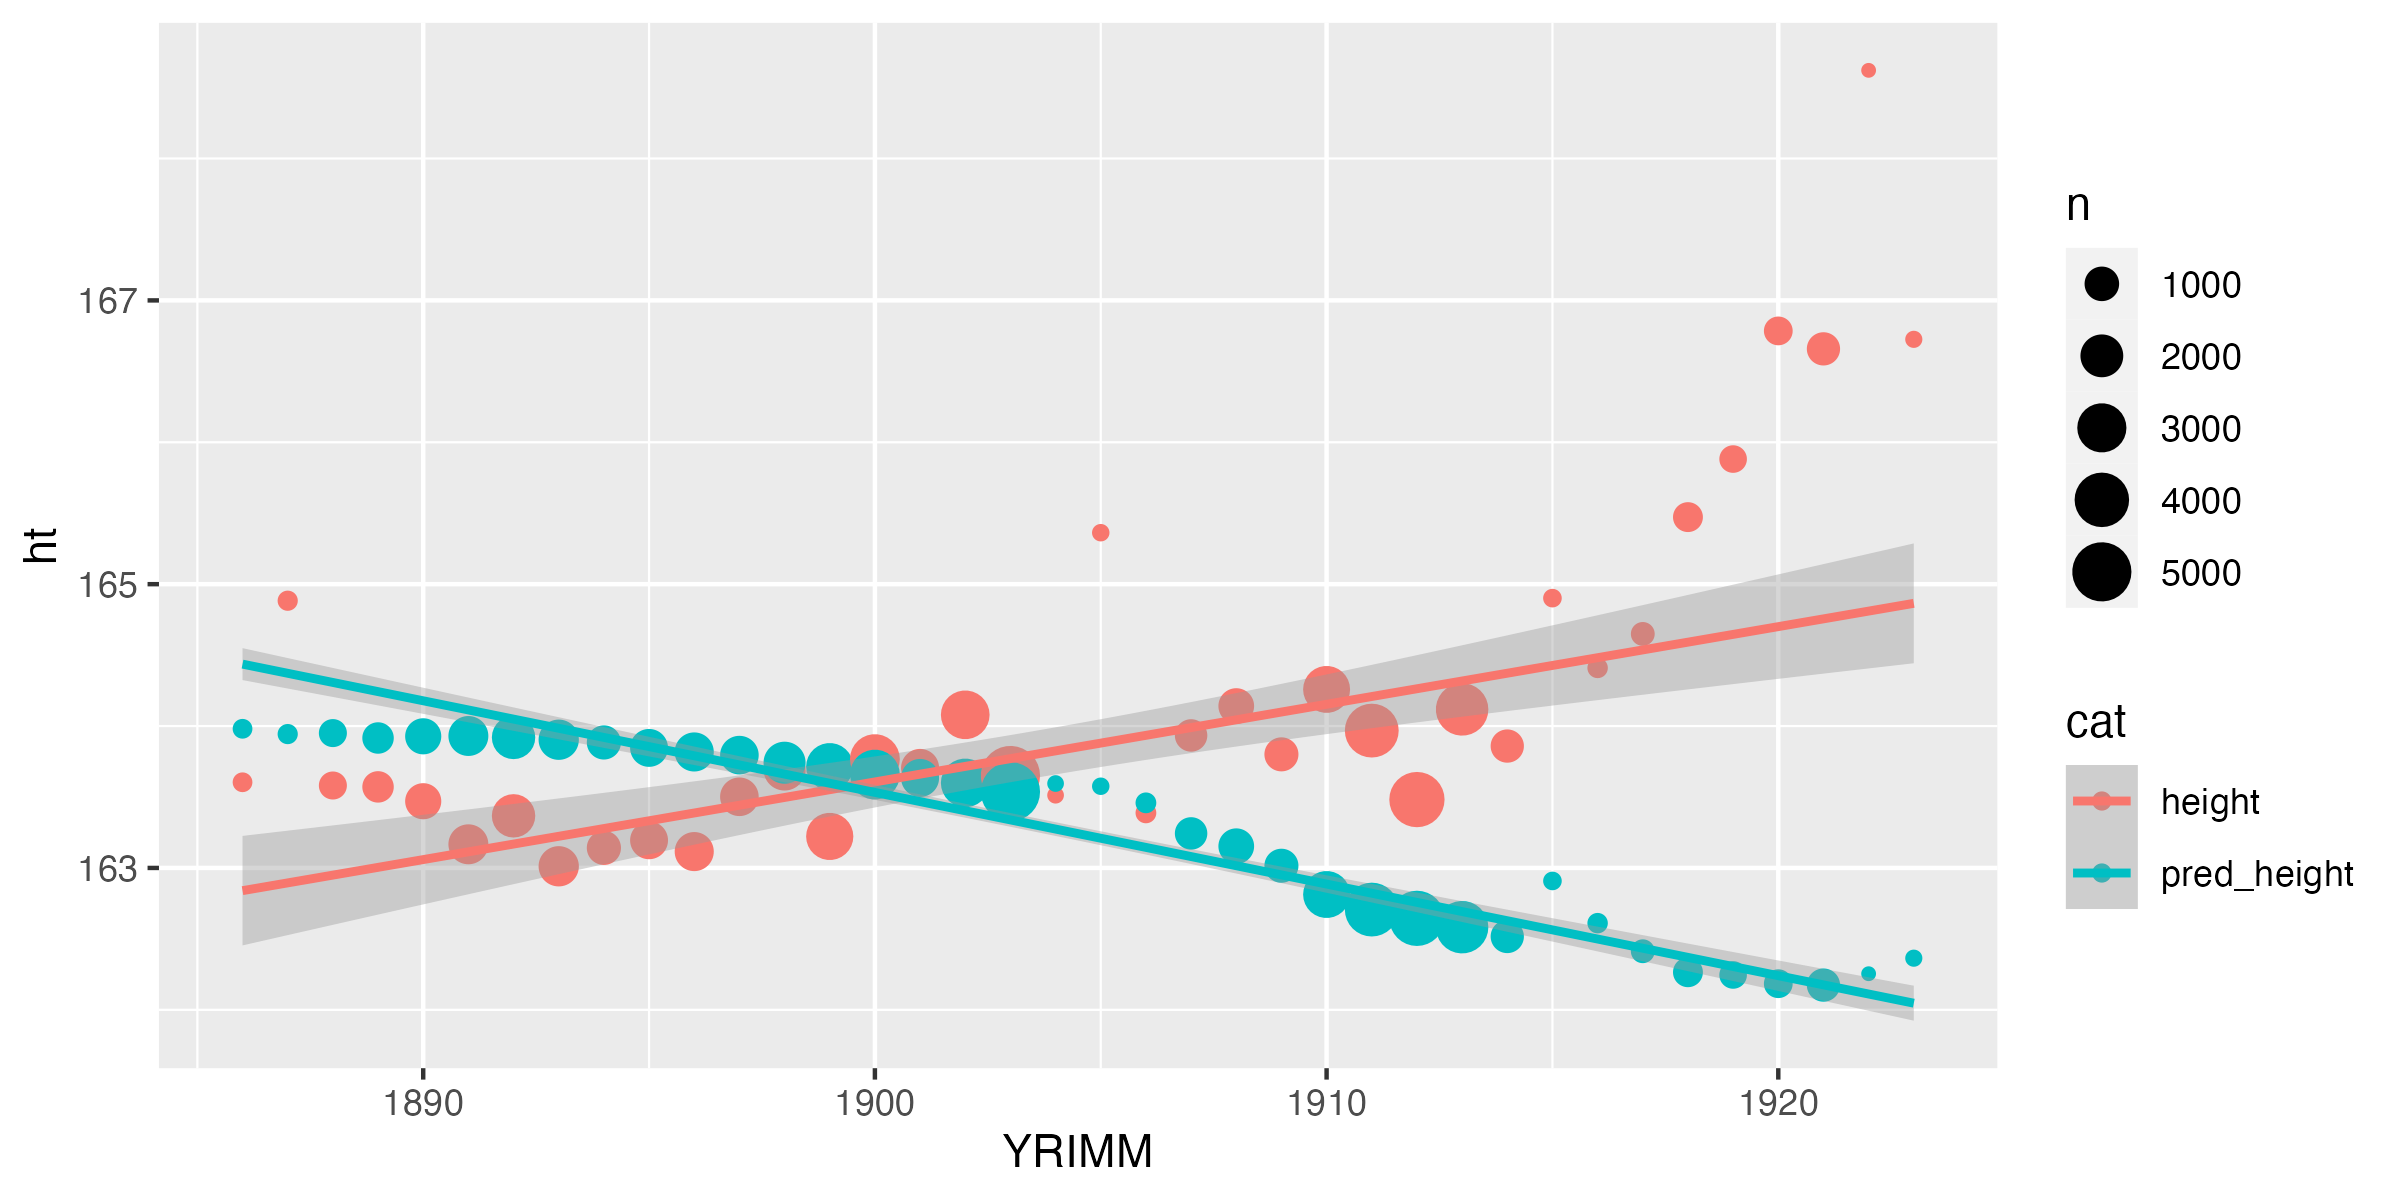
\includegraphics[width=\textwidth]{../../figs/5oct23/heightplot2.png}
    \end{figure}
\end{frame}

\begin{frame}
    \frametitle{Selection on Numeracy: Summary of Results}
    \label{whipple}
    \begin{itemize}
        \item Descriptive evidence of age heaping (tendency to report ages ending in 5 or 0) \hyperlink{agehist}{\beamergotobutton{Histogram: Register}} \hyperlink{agehist_censusall}{\beamergotobutton{Histogram: Census (All Imm)}} \hyperlink{agehist_census}{\beamergotobutton{Histogram: Census (Chinese Imm)}}
        \vspace{2mm}
        \item \textbf{Key Metric:} $whipple = 500 \times \frac{\text{\# ppl age 23-62 w/ age ending in 0 or 5}}{\text{total \# ppl age 23-62}}$ 
        \vspace{2mm}
        \item \textbf{Results from Data:} Increase in numeracy (decrease in whipple) of Chinese imm. over time \hyperlink{whippleplot1}{\beamergotobutton{Whipple Plot}}, esp. relative to other immigrants \hyperlink{whippleplot3_census}{\beamergotobutton{Whipple Plot (Census)}} \vspace{2mm}
        \item \textbf{Results from Baten et al. 2010:} Rapid incr. in numeracy of birth cohorts from 1850-1890 (younger Chinese men are much less likely to round ages) \hyperlink{batenwhipple}{\beamergotobutton{Figure from Paper}} \vspace{2mm}
        \item \textbf{Implication:} contrary (?) to height results -- slightly increasingly \textit{negative} selection on numeracy, as seen by plotting predicted whipple using Baten et al. (2010) again
    \end{itemize}
\end{frame}

\begin{frame}
    \frametitle{Annual Mean Whipple and Mean Predicted Whipple (Register)}
    \begin{figure}
        \centering
        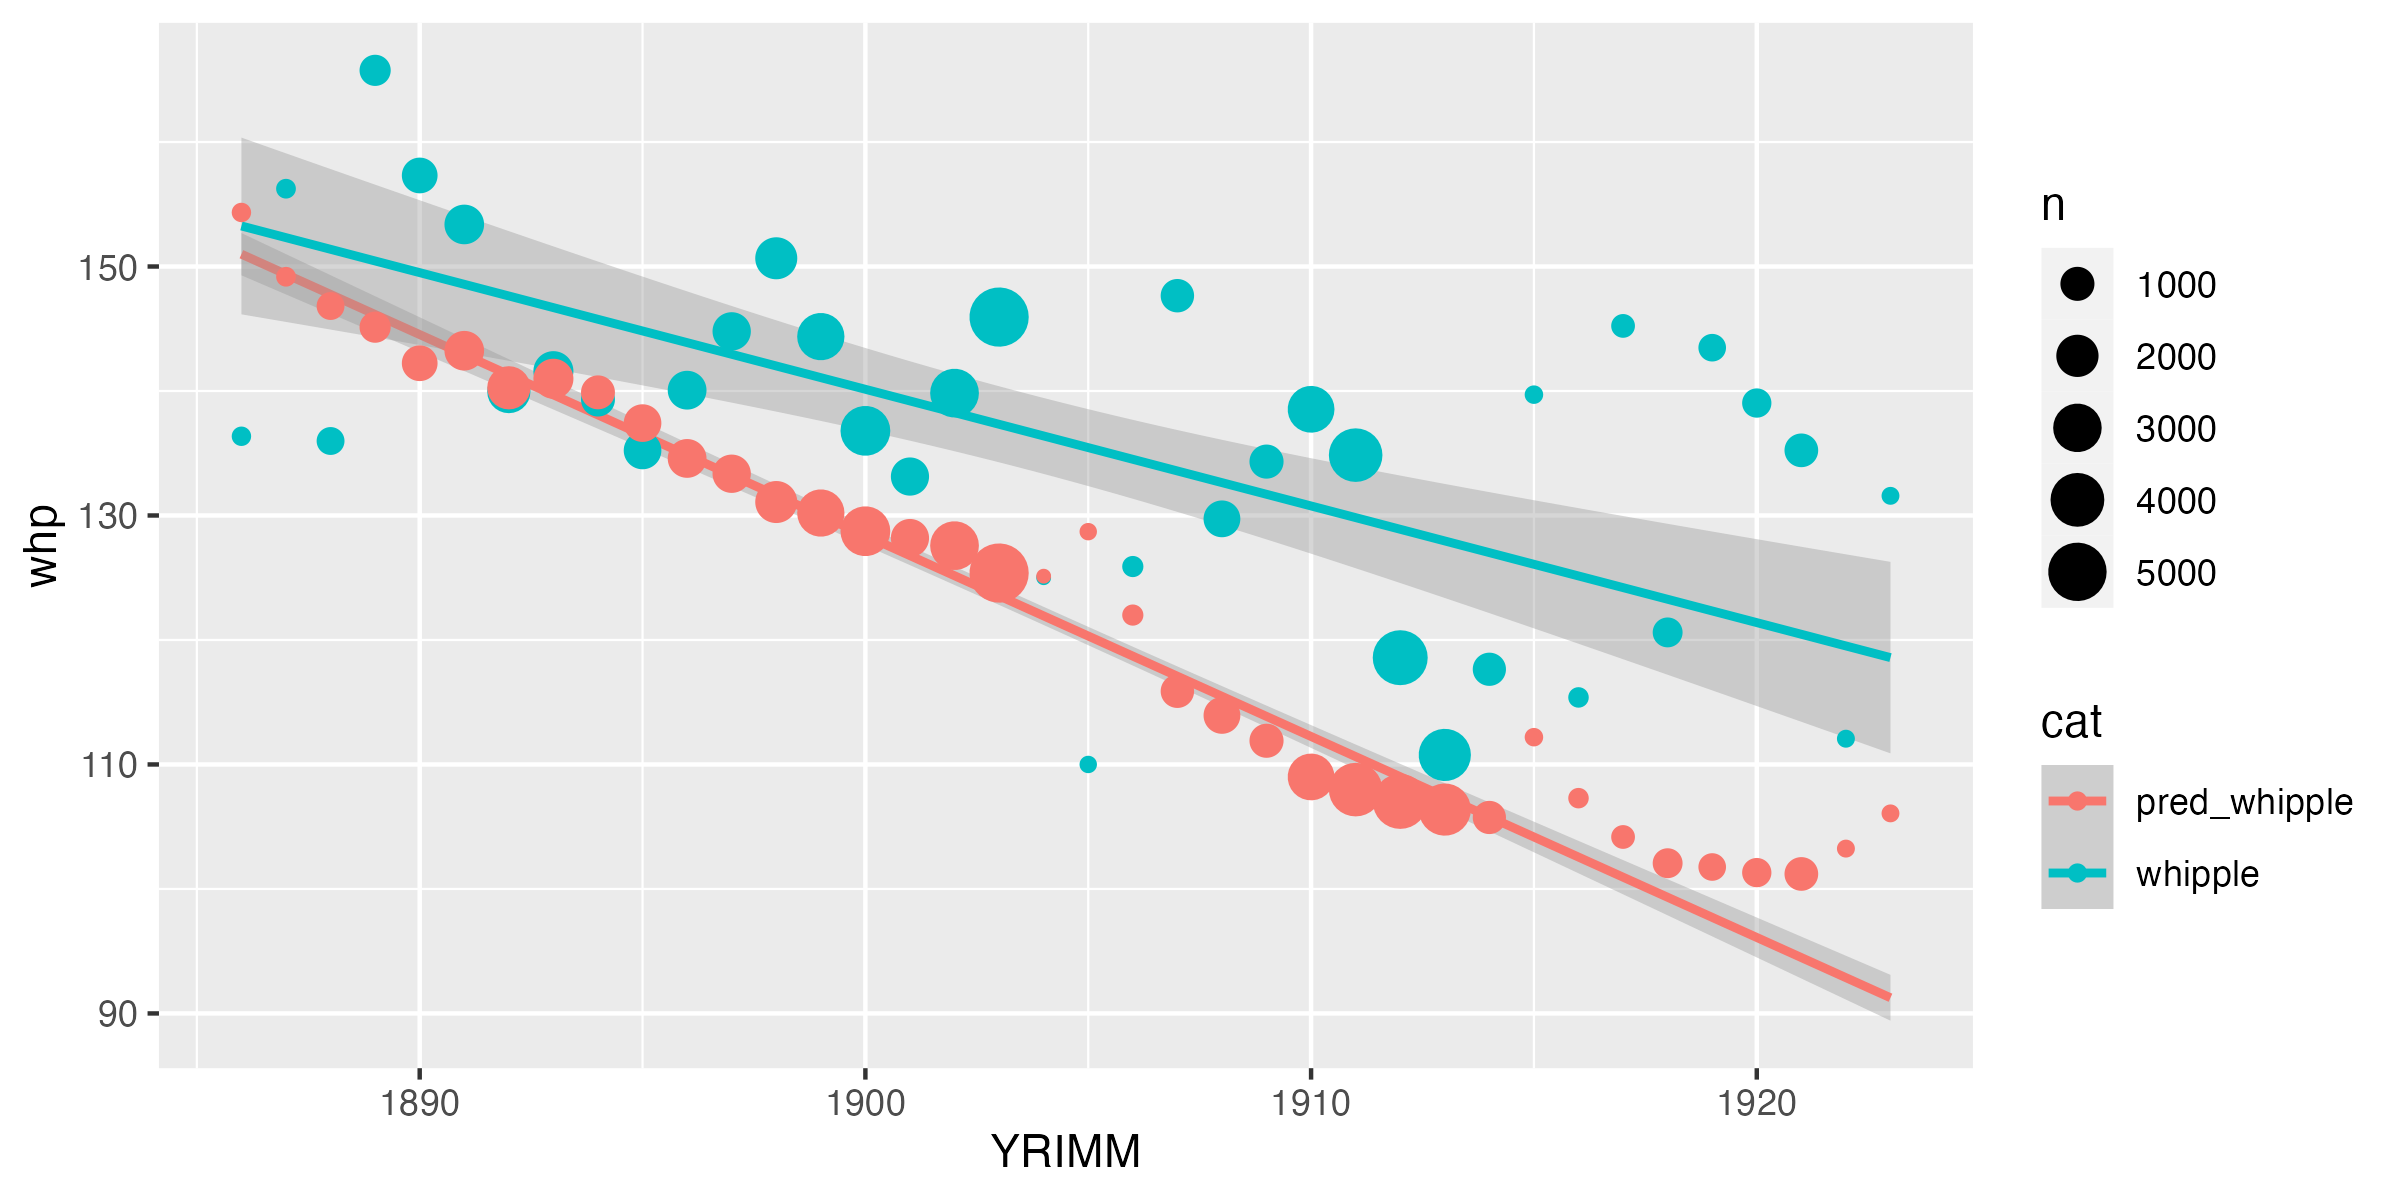
\includegraphics[width=\textwidth]{../../figs/5oct23/whippleplot2.png}
    \end{figure}
\end{frame}

\begin{frame}
    \frametitle{Results on Selection: Takeaways?}
    \begin{itemize}
        \item Main conclusions drawn from comparison with Baten et al. 2010 paper, which I don't have the data for [yet?]
        \item Mostly reinforce takeaway of positive selection that I also find in Census (on occupation and literacy)
        \item Numeracy results a bit puzzling (esp. compared to literacy in the census)
        \item How to tie back to head tax? or is it fine to show trends over this period as descriptive?
    \end{itemize}
\end{frame}

\section{Intro and First Stage Drafts}
\begin{frame}
    \frametitle{Framing Project}
        \textbf{Option 1:} Big-picture framing, main focus on what we can learn about immigration more generally from this one historical episode 
        \begin{itemize}
            \item references: Feigenberg (2020) on effect of border fence construction on selection [present day, Mexico]; Escamilla-Guerrero and López-Alonso (2023) on effect of 1907 crisis on selection [historical, Mexico]
            \item not sure how my work necessarily contributes to the existing literature, other than to look at a different group of immigrants \& using cool data 
            \item other papers do have exogenous shocks to migration cost (if not explicitly in monetary terms) 
            \item i find more positive selection due to HT -- what is the policy implication?
        \end{itemize}
\end{frame}

\begin{frame}
    \frametitle{Framing Project}
    \textbf{Option 2:} More narrow framing, main focus is on documenting trends in Chinese immigration under the Chinese Head Tax
        \begin{itemize}
            \item references: Kanazawa (2005) on political economy of Chinese exclusion
            \item less general-interest, likely harder to publish 
            \item closer to the reason I was interested in this topic in the first place, more emphasis on how horrible this tax was 
        \end{itemize}
\end{frame}

%%%%%%%%%%%%%%%%%%%%%%%%%%%%%%%%%
\appendix 
\begin{frame}
    \label{heightplot1}
    \frametitle{Raw Annual Mean Height \hyperlink{height}{\beamerreturnbutton{Back}}}
    \begin{figure}
        \centering
        
\includegraphics[width=\textwidth]{../../figs/5oct23/heightplot1.png}
    \end{figure}
\end{frame}

\begin{frame}
    \label{ageplot1}
    \frametitle{Raw Annual Mean Age \hyperlink{height}{\beamerreturnbutton{Back}}}
    \begin{figure}
        \centering
        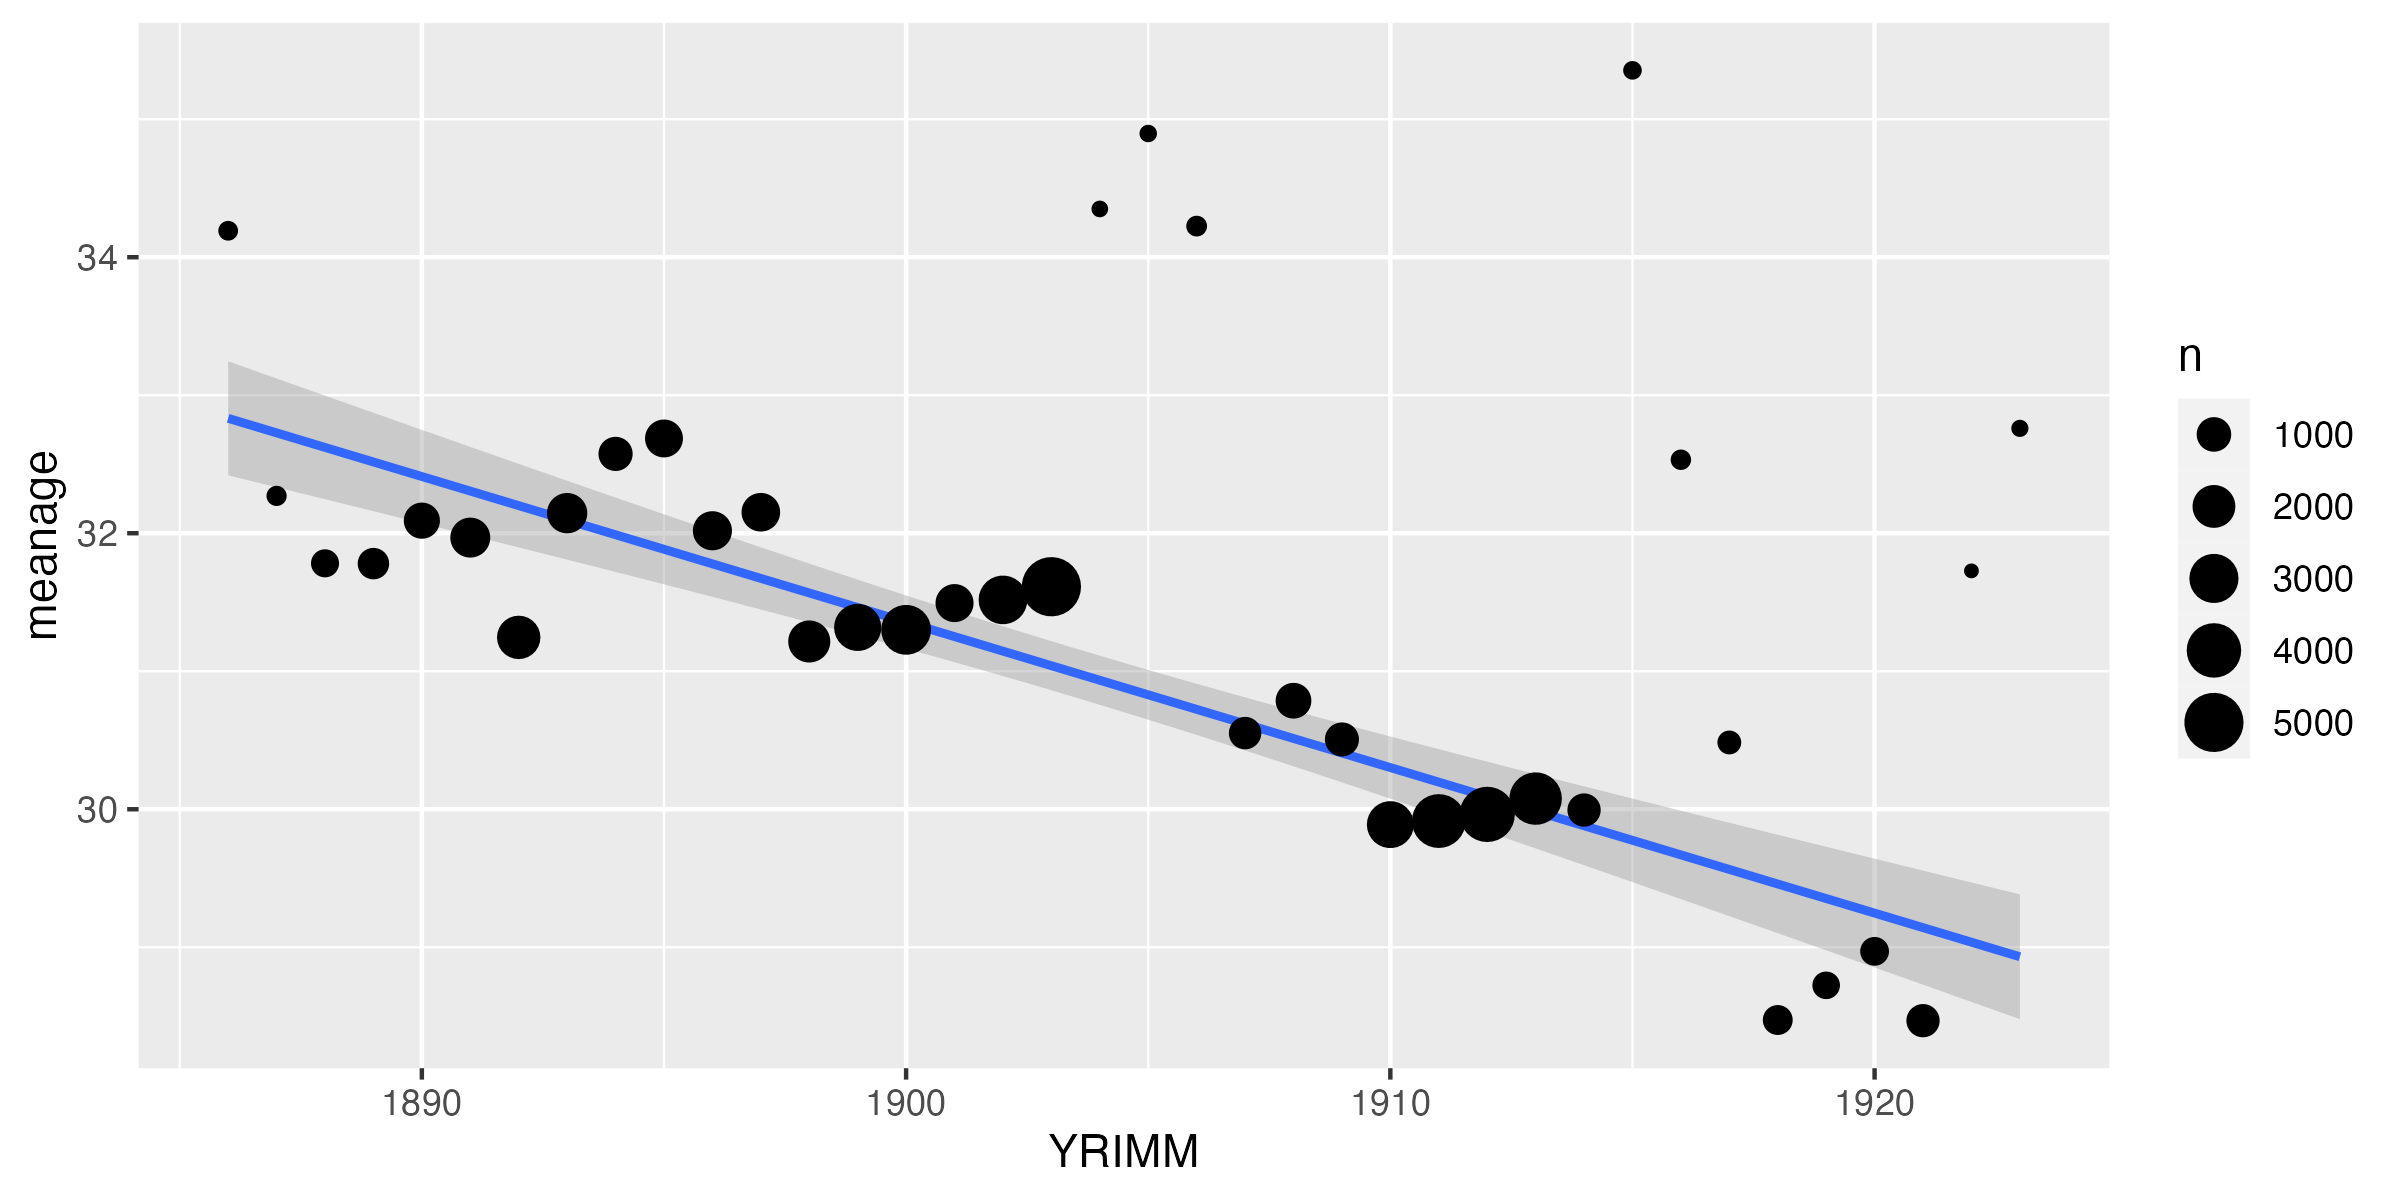
\includegraphics[width=\textwidth]{../../figs/5oct23/ageplot1.png}
    \end{figure}
\end{frame}

\begin{frame}
    \frametitle{Baten et al. 2010 Height Patterns \hyperlink{height}{\beamerreturnbutton{Back}}}
    \label{batenheight}
    \begin{figure}
        \centering
        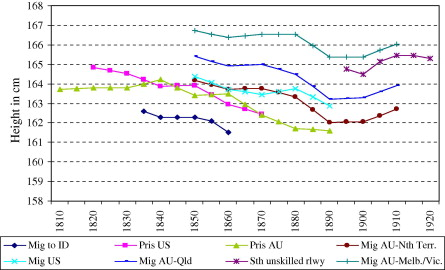
\includegraphics[width=0.7\textwidth]{../../figs/5oct23/batenetal2010_height.jpg}
    \end{figure}
\end{frame}

\begin{frame}
    \frametitle{Histogram of Ages in Chinese Register \hyperlink{whipple}{\beamerreturnbutton{Back}}}
    \label{agehist}
    \begin{figure}
        \centering
        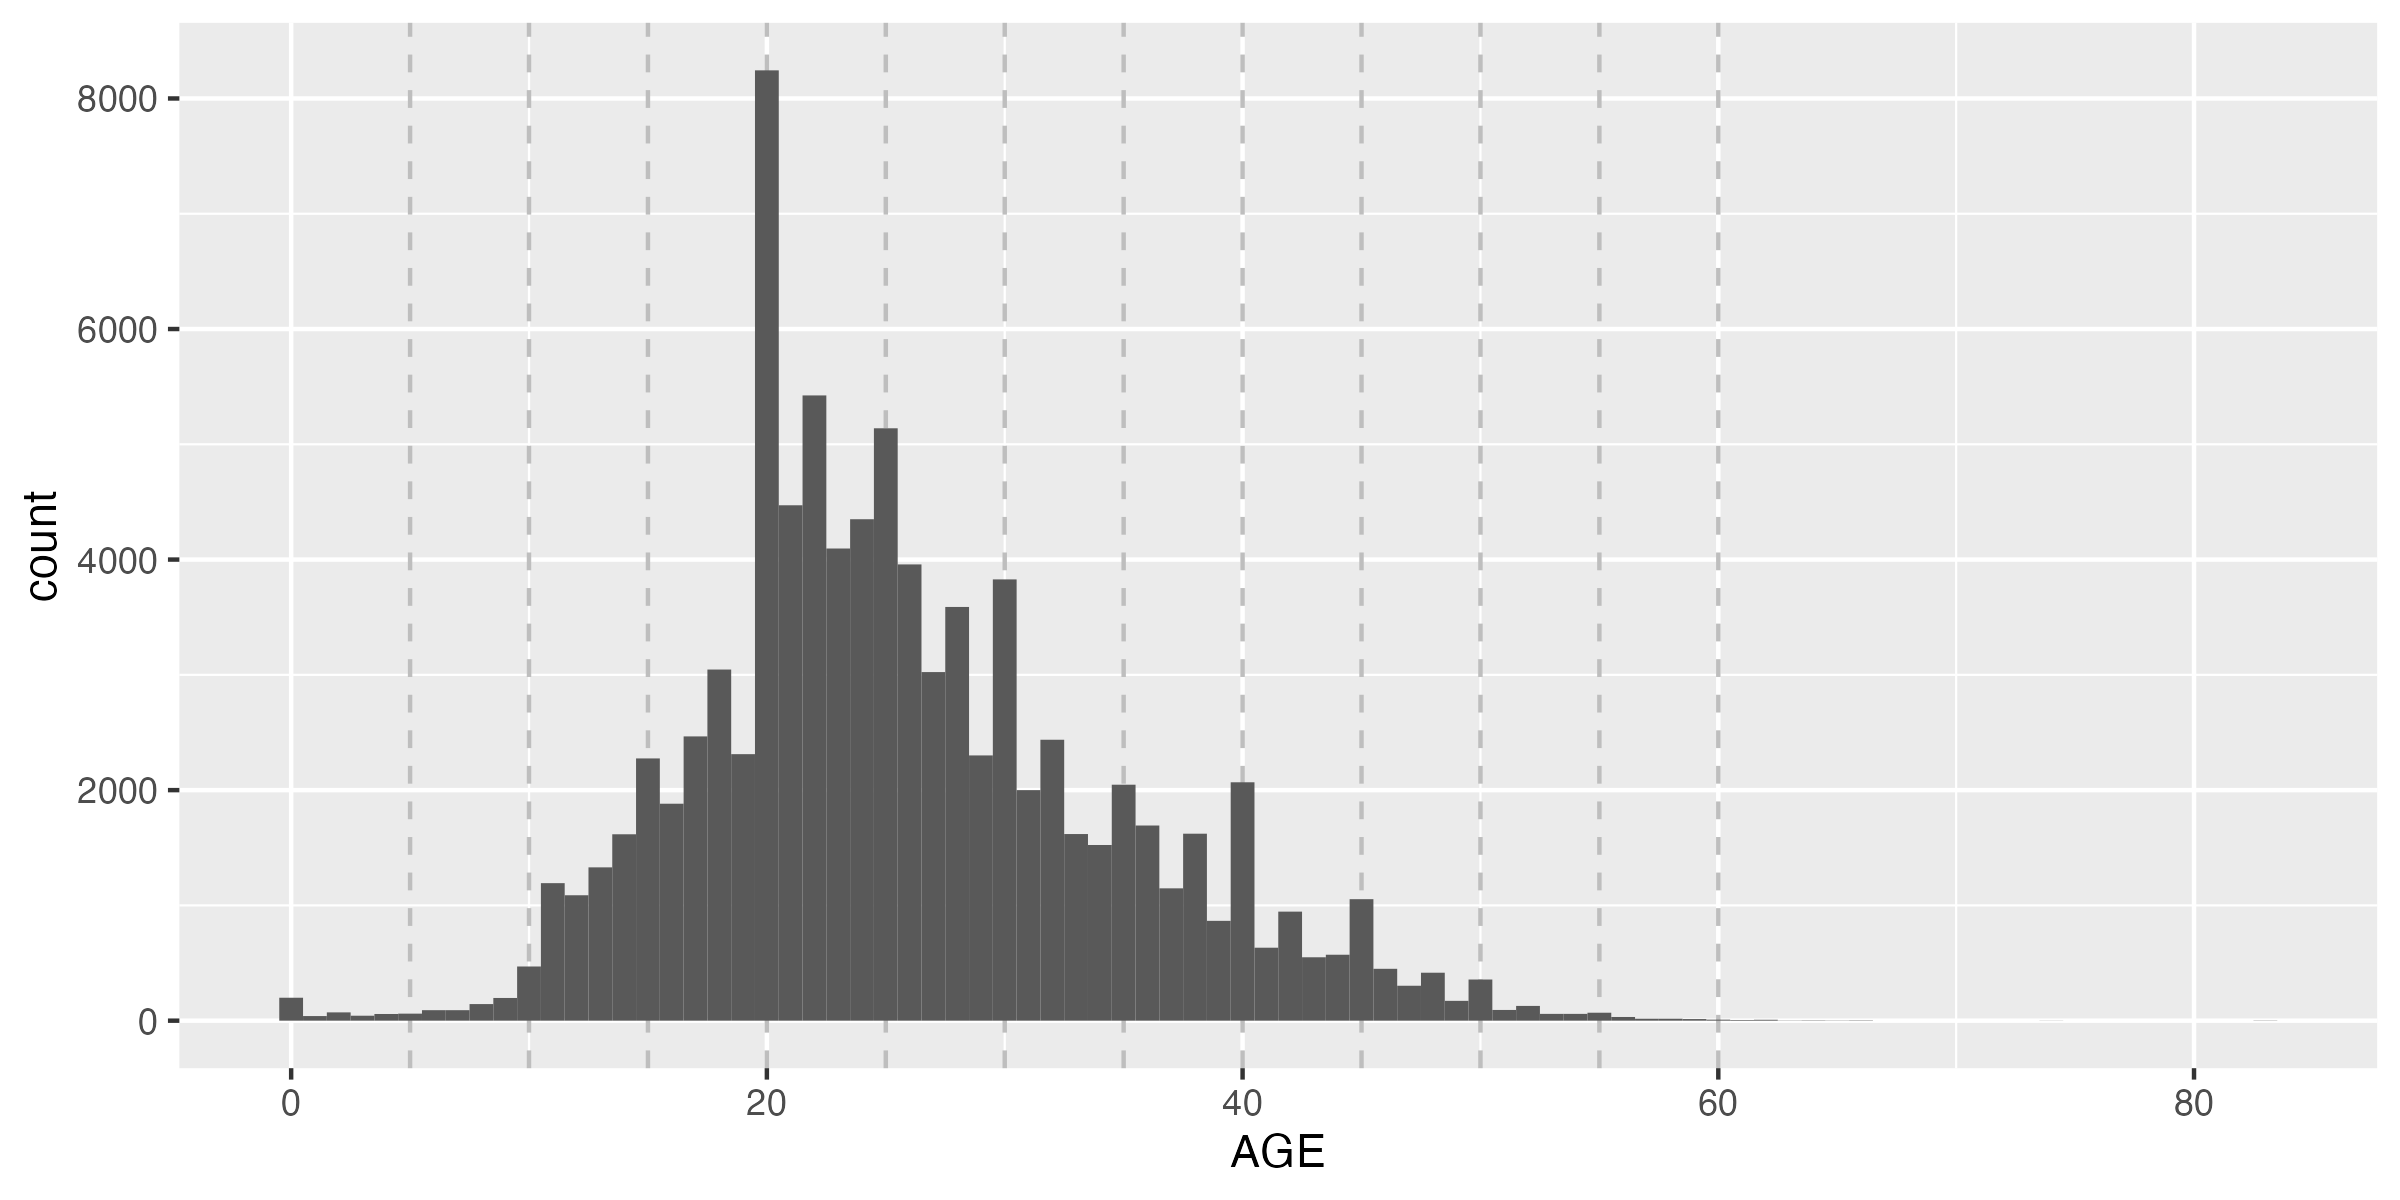
\includegraphics[width=\textwidth]{../../figs/5oct23/agehist.png}
    \end{figure}
\end{frame}

\begin{frame}
    \frametitle{Histogram of Ages in Canadian Census: All Immigrants \hyperlink{whipple}{\beamerreturnbutton{Back}}}
    \label{agehist}
    \begin{figure}
        \centering
        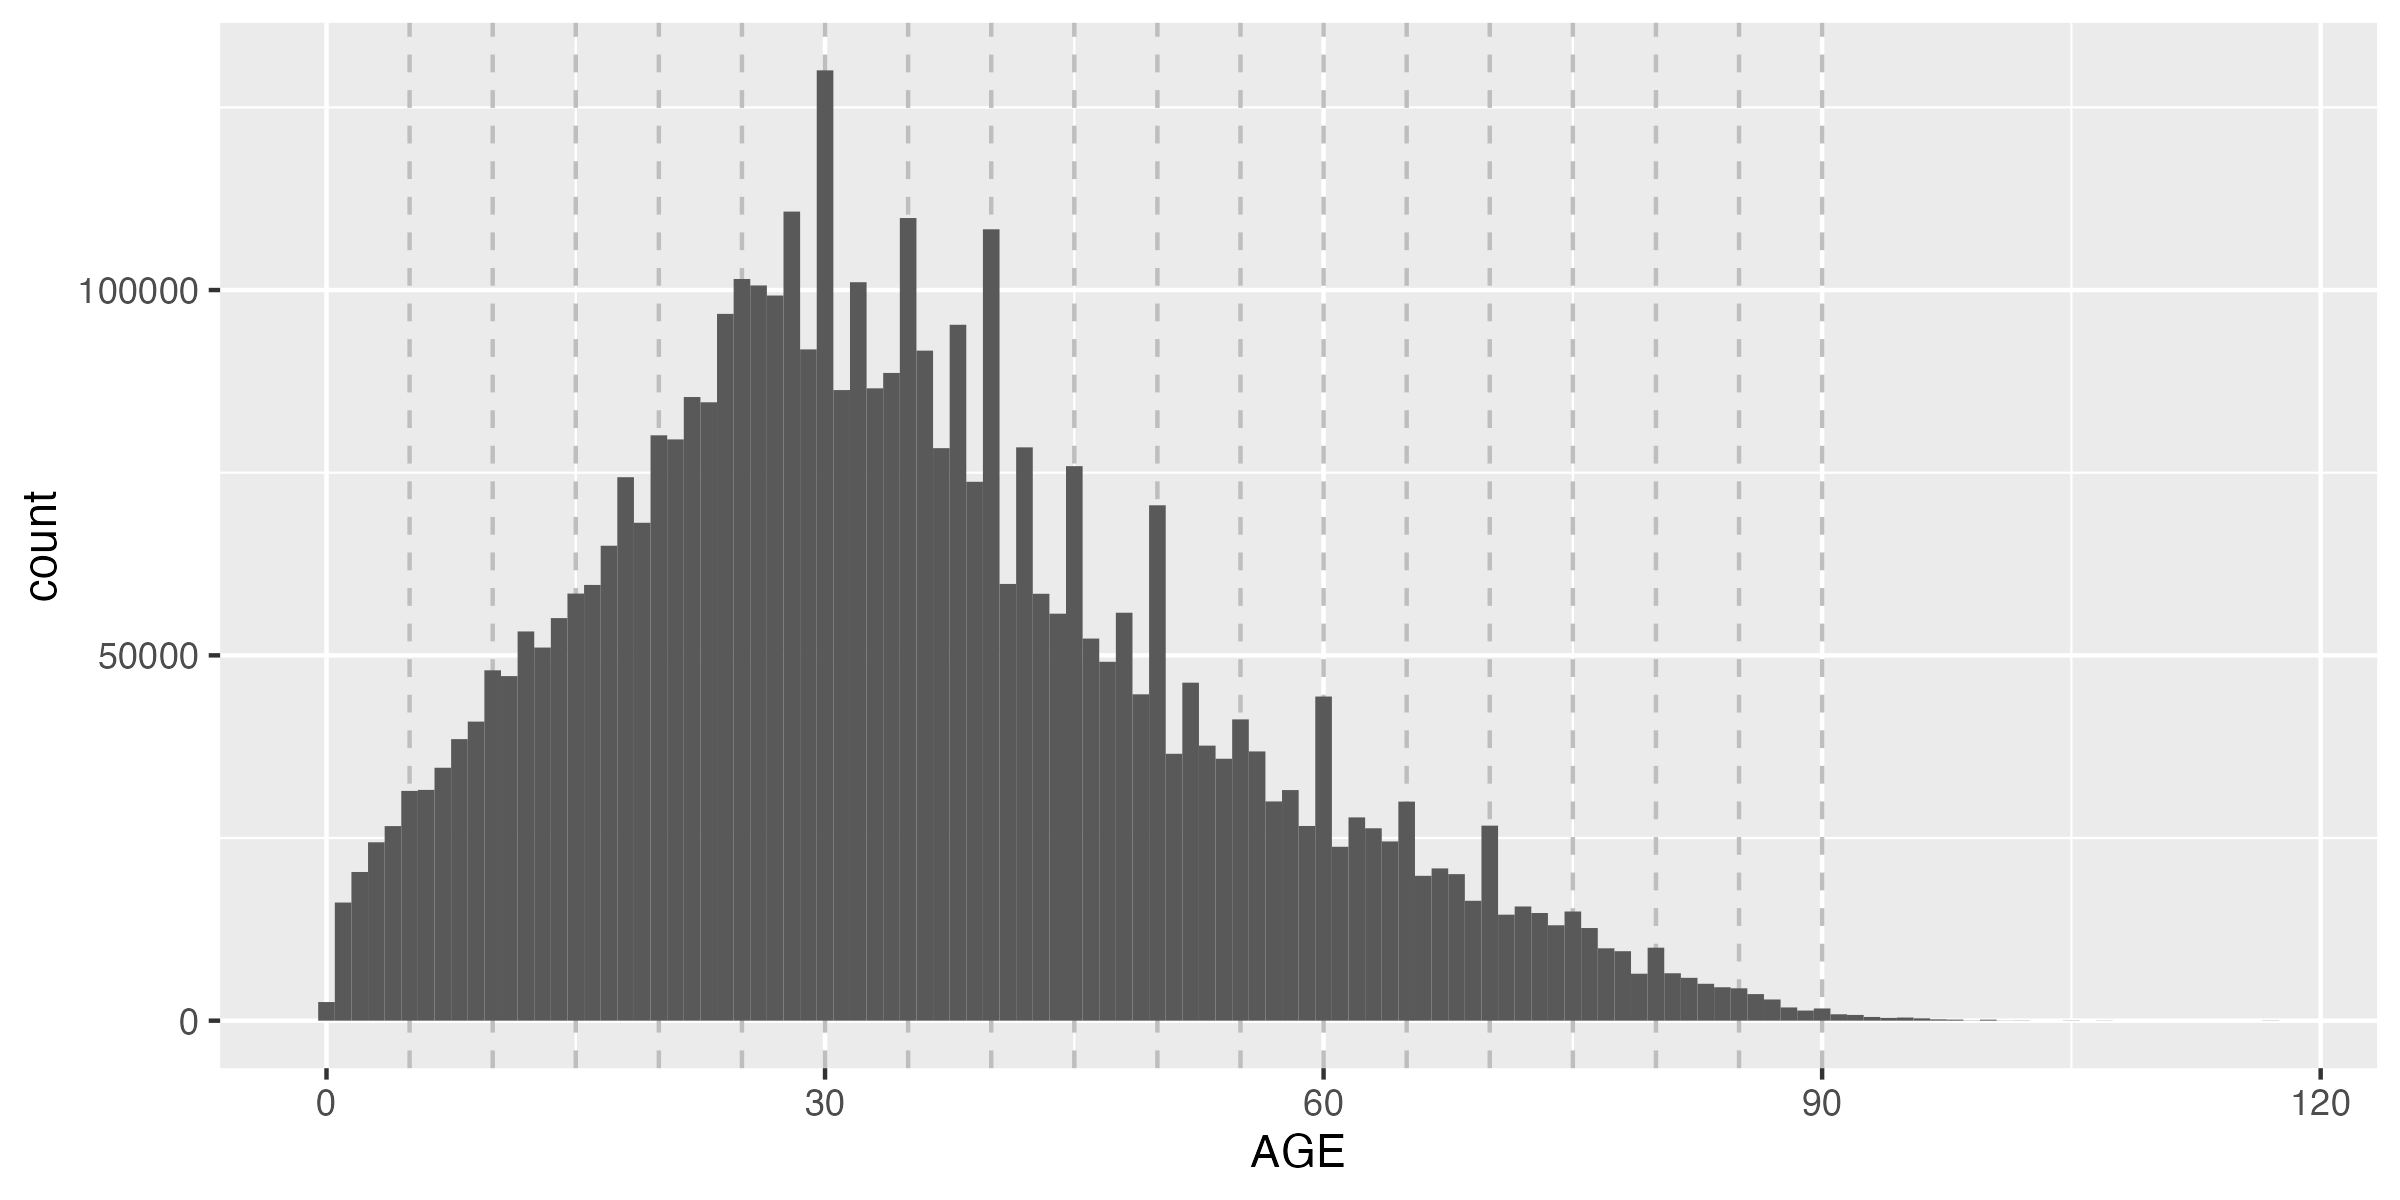
\includegraphics[width=\textwidth]{../../figs/5oct23/agehist_censusall.png}
    \end{figure}
\end{frame}

\begin{frame}
    \frametitle{Histogram of Ages in Canadian Census: Chinese Immigrants \hyperlink{whipple}{\beamerreturnbutton{Back}}}
    \label{agehist}
    \begin{figure}
        \centering
        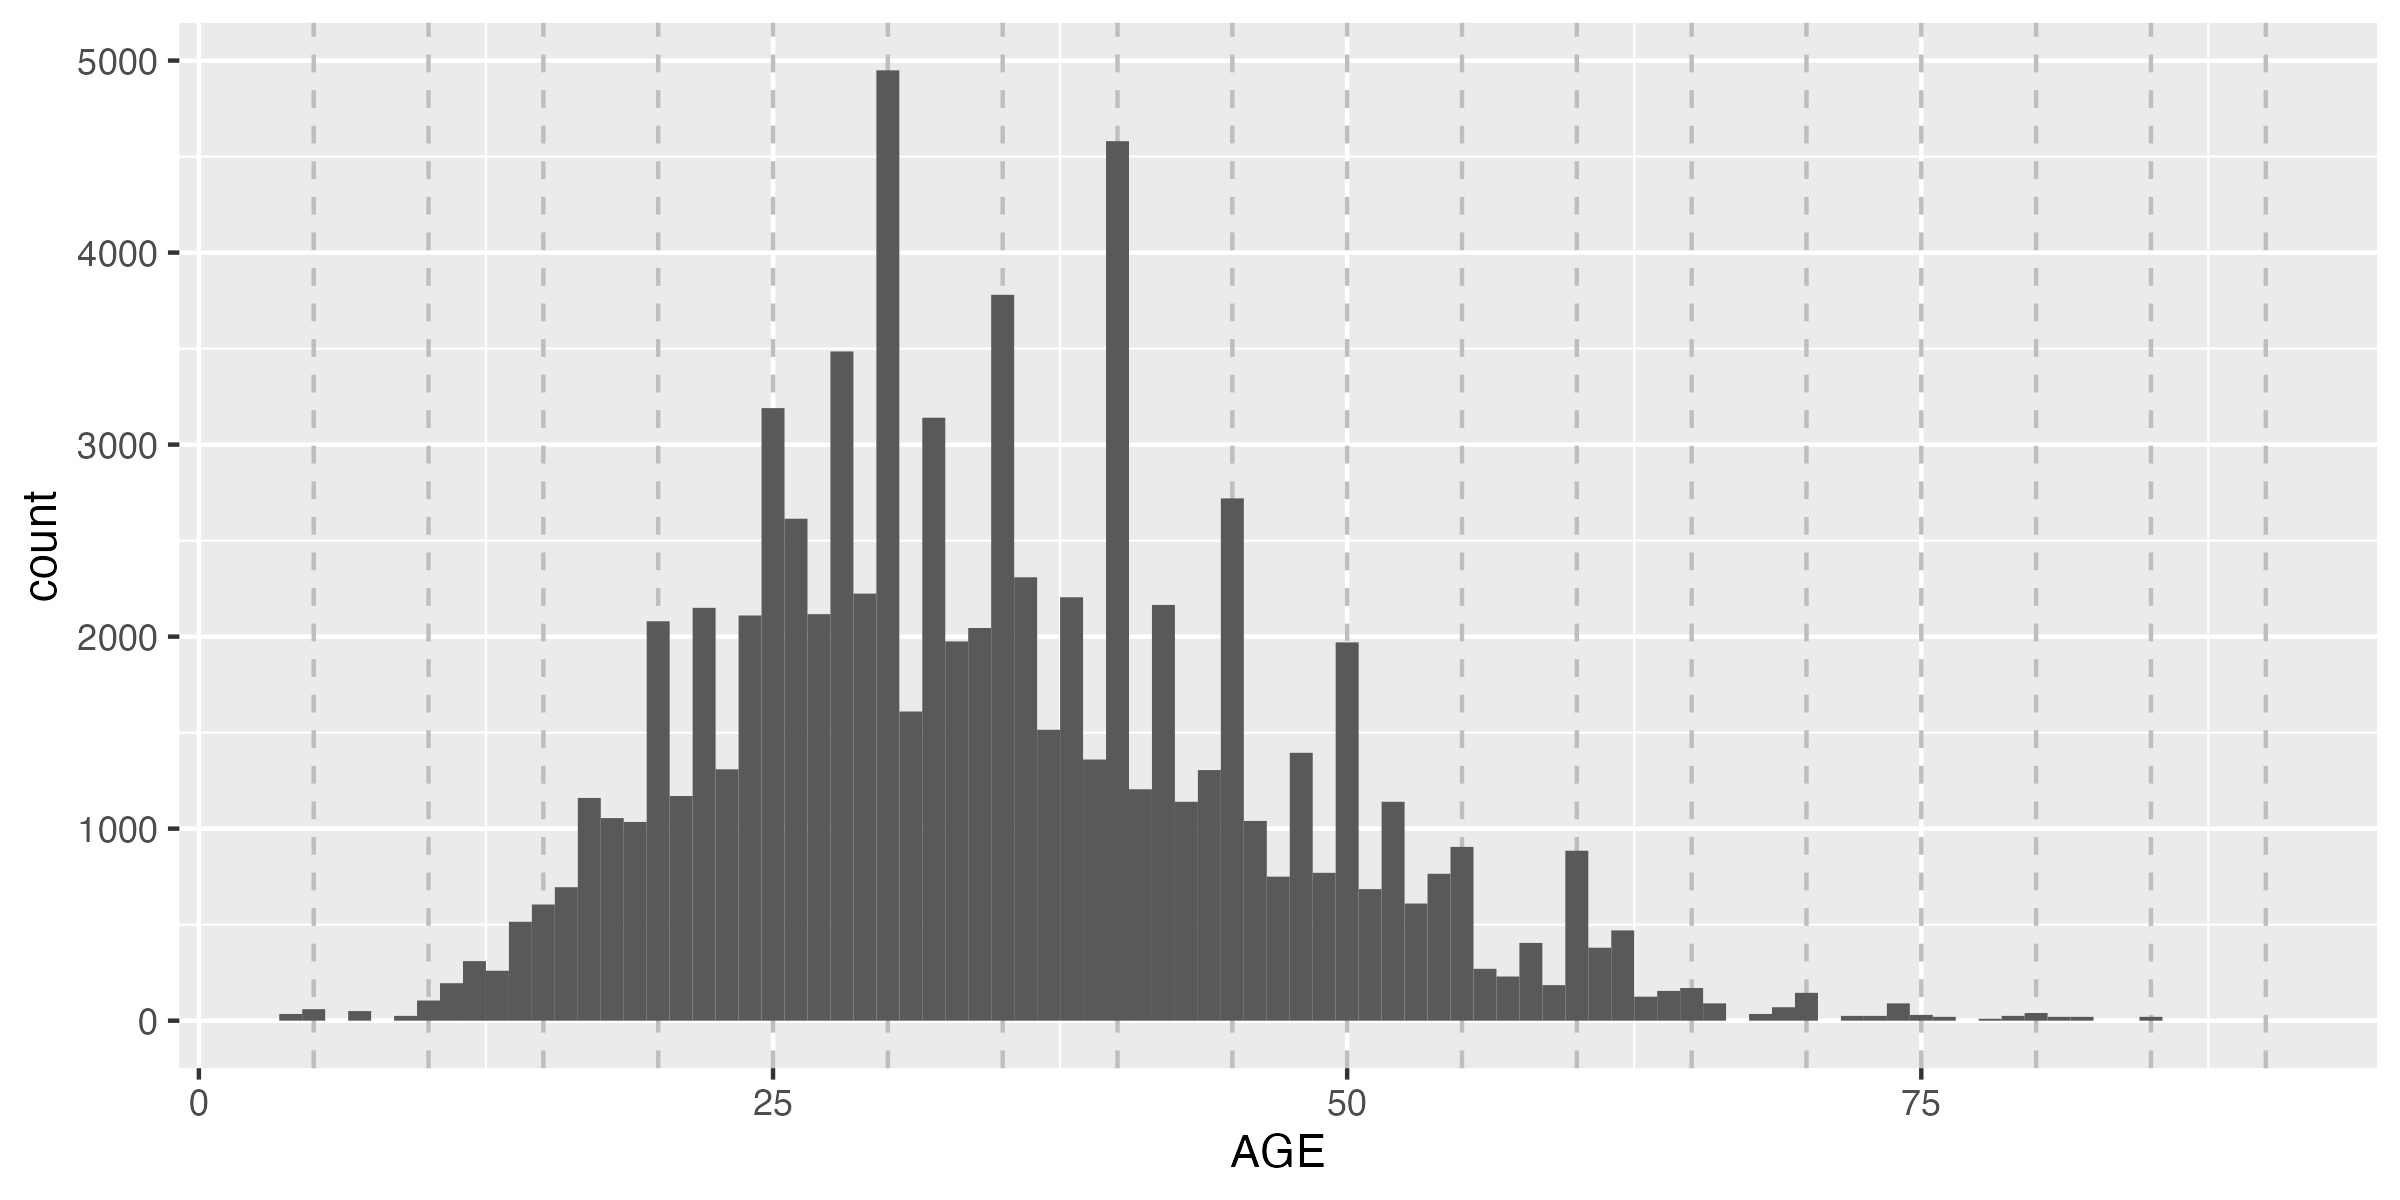
\includegraphics[width=\textwidth]{../../figs/5oct23/agehist_census.png}
    \end{figure}
\end{frame}

\begin{frame}
    \label{whippleplot1}
    \frametitle{Raw Annual Mean Whipple Index (Register) \hyperlink{whipple}{\beamerreturnbutton{Back}}}
    \begin{figure}
        \centering
        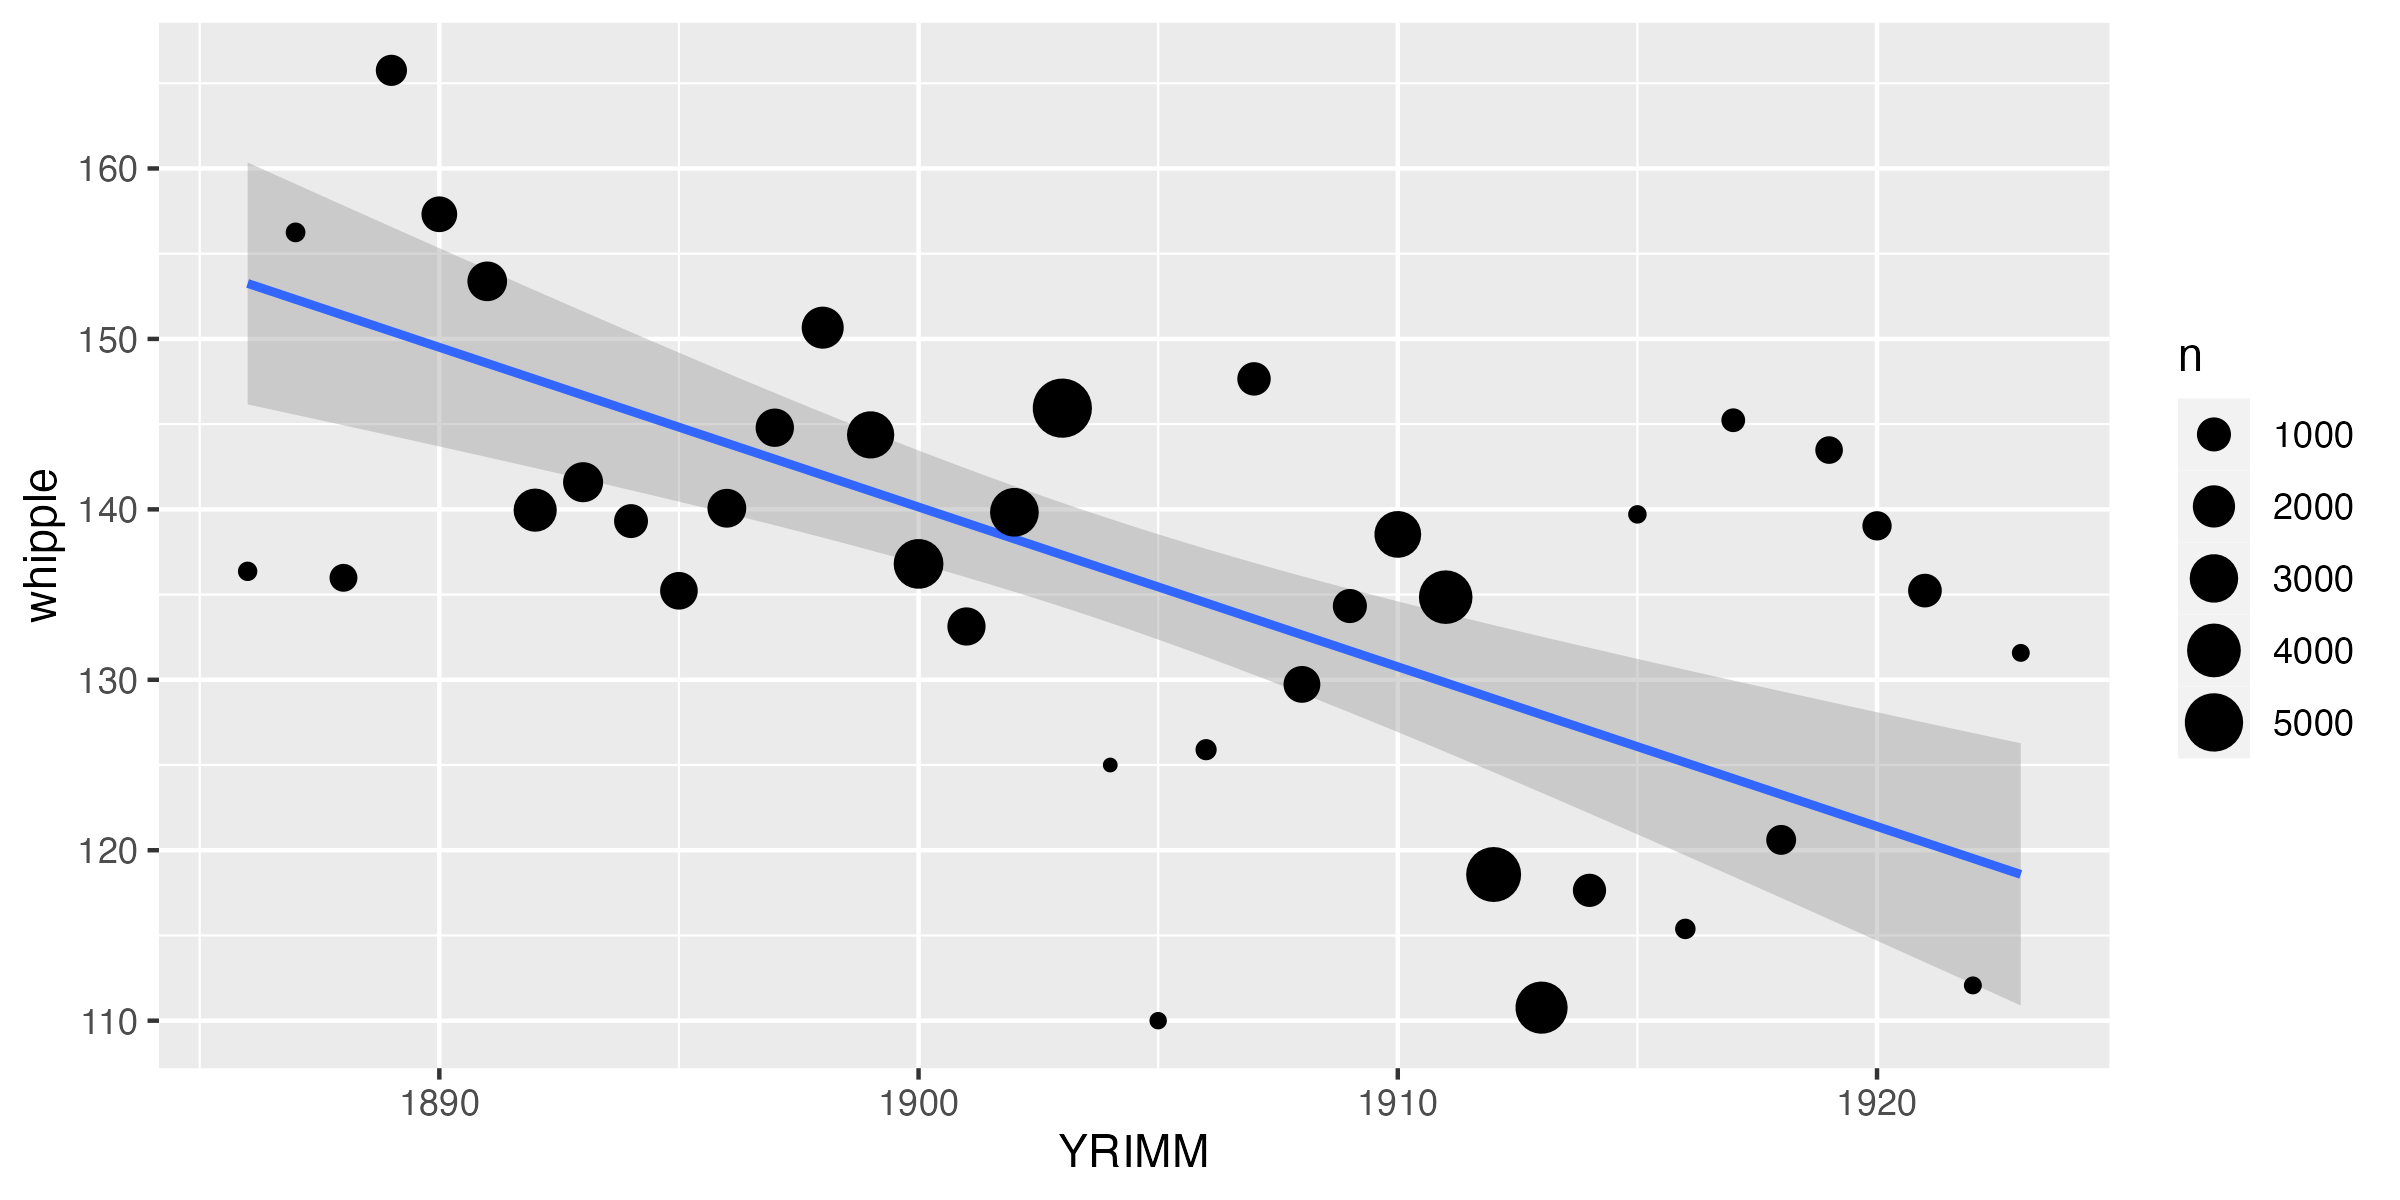
\includegraphics[width=\textwidth]{../../figs/5oct23/whippleplot1.png}
    \end{figure}
\end{frame}

\begin{frame}
    \label{whippleplot3_census}
    \frametitle{Whipple Index for Chinese vs. Non-Chinese Imm. (Census) \hyperlink{whipple}{\beamerreturnbutton{Back}}}
    \begin{figure}
        \centering
        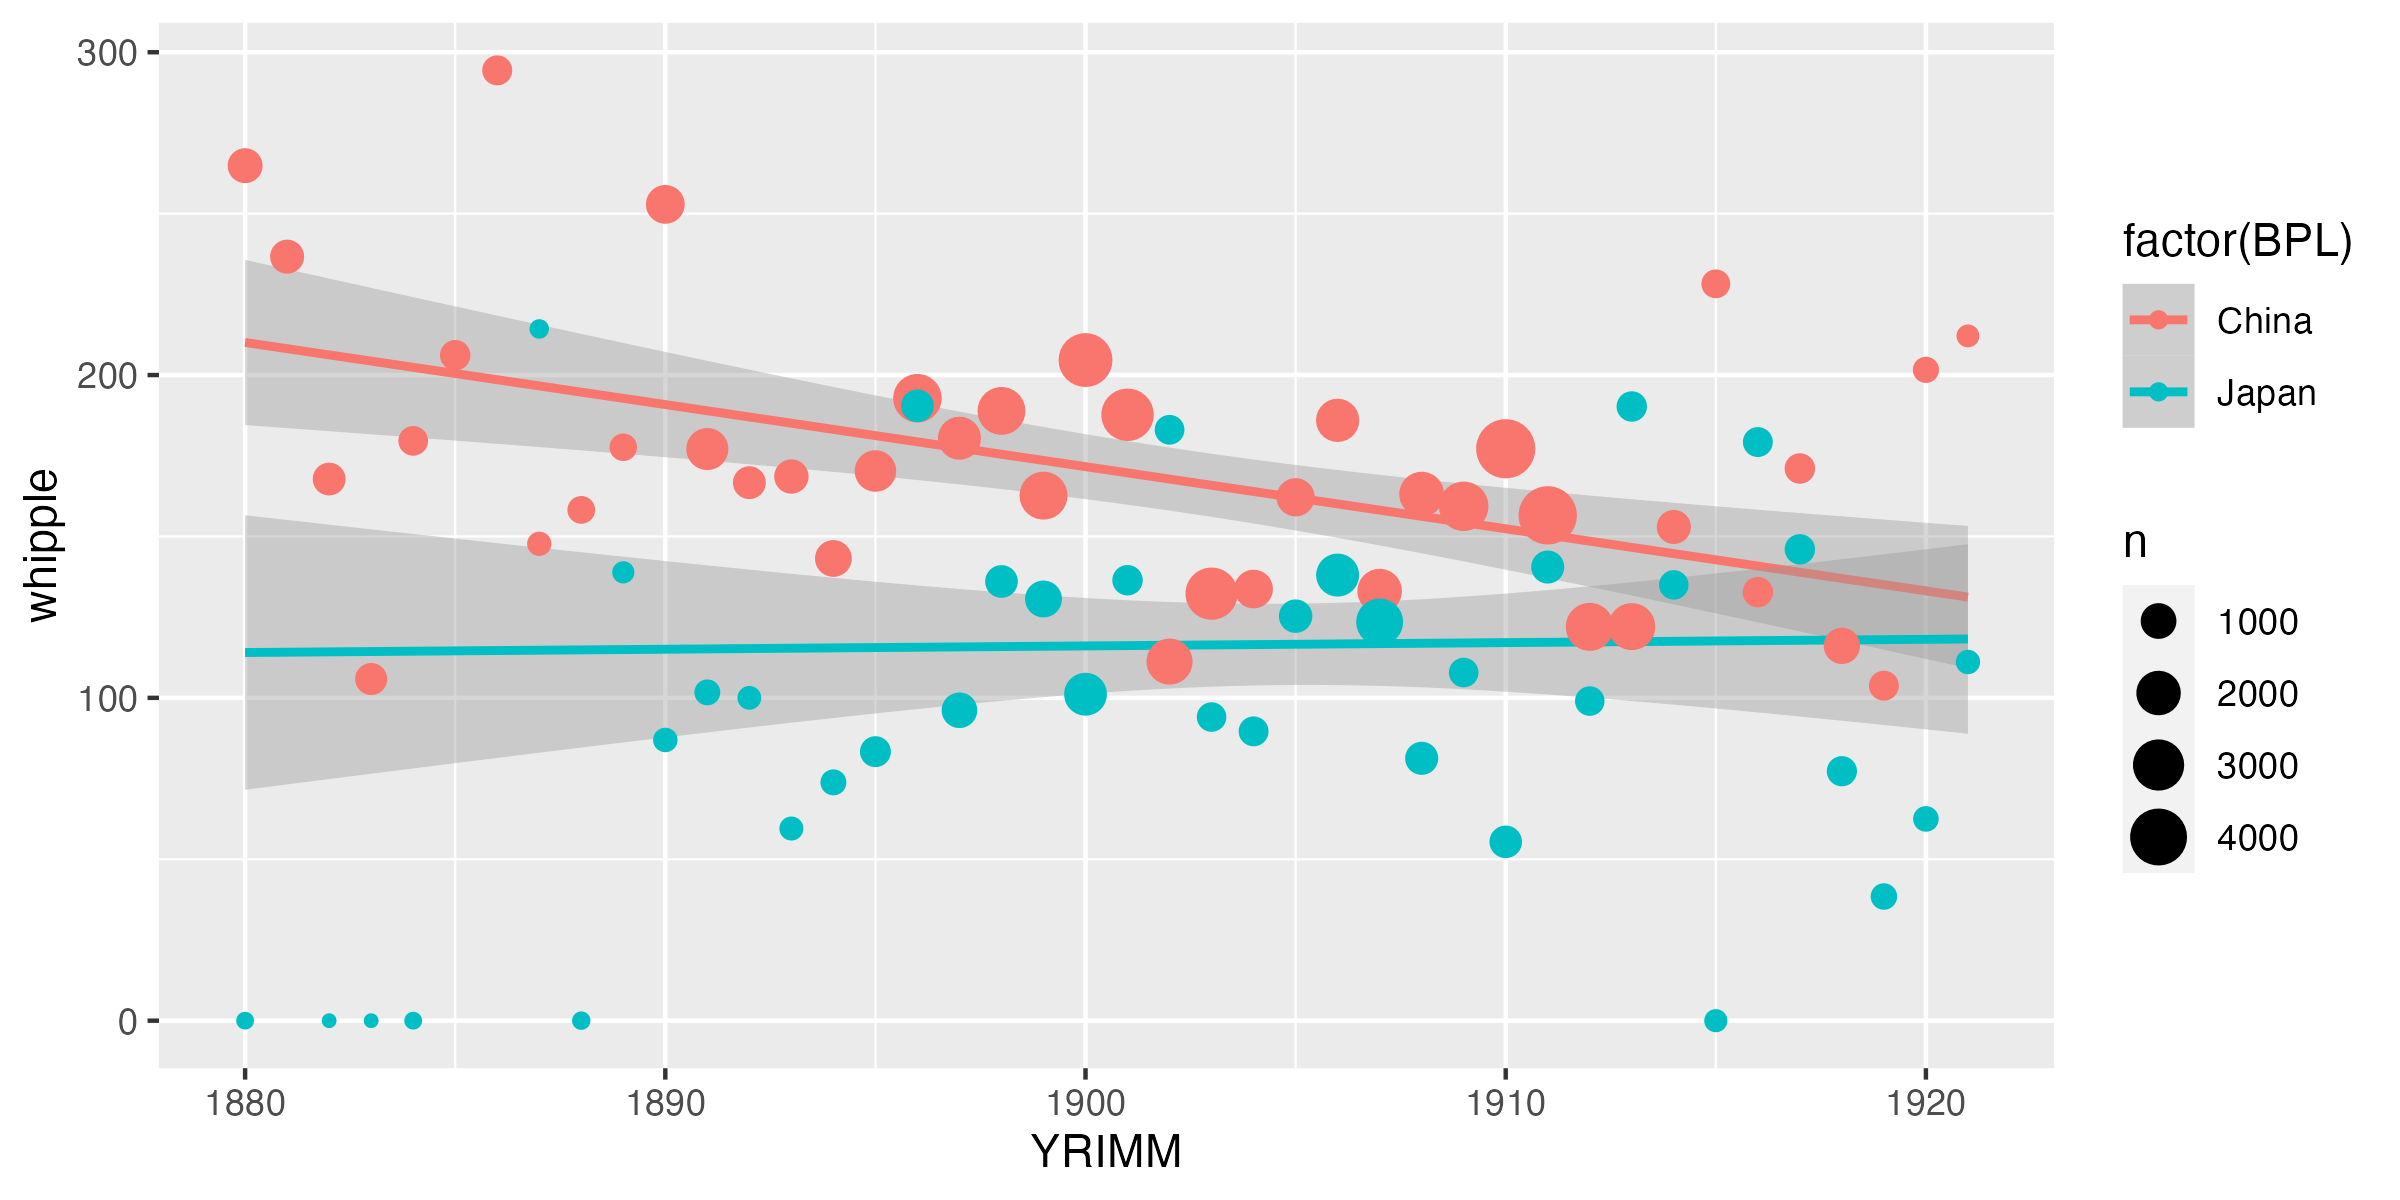
\includegraphics[width=\textwidth]{../../figs/5oct23/whippleplot3_census.png}
    \end{figure}
\end{frame}

\begin{frame}
    \frametitle{Baten et al. 2010 Whipple Patterns \hyperlink{whipple}{\beamerreturnbutton{Back}}}
    \label{batenwhipple}
    \begin{figure}
        \centering
        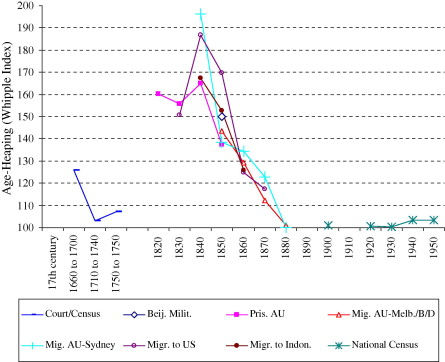
\includegraphics[width=0.5\textwidth]{../../figs/5oct23/batenetal2010_whipple.jpg}
    \end{figure}
\end{frame}

\end{document}